\documentclass[10pt]{beamer}
\usepackage{listings}
\usetheme{uha}
\usepackage{hyperref}
\usepackage{indentfirst}
\usepackage{booktabs}
\usepackage{multirow}
\usepackage{xeCJK}
\usepackage[french,english]{babel}
\usepackage[T1]{fontenc}
\usepackage[utf8]{inputenc}
\usepackage{amsmath}
\usepackage{amsfonts}
\usepackage{amssymb}
\usepackage{tikz}
\setmainfont{Ubuntu}
\title{Five Years Plan}
\subtitle{2019.5-2024.5}
\date{\today}
\author{w:haobo.gao r:yanphy.li}
\institute{ZhengZhou}

\lstset{
	numbers=left,
	numberstyle=\tiny,
	basicstyle=\scriptsize,
	backgroundcolor= \color{gray},
	keywordstyle=\color{blue!70},
	breaklines=true,
	breakautoindent=true,
	breakindent=4em,
	commentstyle=\color{codegreen},
	frame=shadowbox,
	escapeinside=``,
	tabsize=4,
	framextopmargin=1pt,framexbottommargin=1pt,abovecaptionskip=-1pt,belowcaptionskip=1pt,
  xleftmargin=3em,xrightmargin=3em,
	language=C
}


\begin{document}




% Title page 标题页
\begin{frame}[plain, noframenumbering]
	\titlepage
\end{frame}



%=============================================================================================
\section{Introduction}

%------------------------------------------------
\begin{frame}[fragile]{介绍}
		为因应经济及家庭发展之需求,为将来阶段发展赋予可参考之准线。遂制定此五年之计划。

		望双方可以在计划框架下,拥有充分之担当,以及使命感,确保计划的按时达成。
\end{frame}


%------------------------------------------------
\begin{frame}[fragile]{前言}
	从走出校门开始,我们就掌握了人生的方向盘。 有幸 相结为一个unit,一起探索,十分
幸运。
	 学校的教育

	 如果在大学中树立坚定之目标,并为之奋斗。 这样毕业可以成为行业新人中的新锐,并持续 投入
积累。不会存在毕业后不会出现目标确实,迷茫。



\end{frame}

%--------------------------------------------
\begin{frame}[fragile]{一些数据}
		\begin{center}
		\begin{tabular}{|l|c|c|c|c|c|}
		\hline
		年度\& 项目	&	yanphy & 年龄 & haobo & 年龄 & 期望净存 \\
		\hline
		2020 & \_ &	25  &	\_ & 24  &   0  \\
		2021 & \_ & 26	& \_ & 25  &     \\
		2022 & \_ & 27  & \_ & 26  &     \\
		2023 & \_ & 28  & \_ & 27  &     \\
		2024 & \_ & 29  & \_ & 28  &     \\
		\hline
		\end{tabular}
		\end{center}
		2020 年度是指 2019.5-2020.5 为第一个年度
		2021 年度是指 2020.5-2021.5 为第二个年度

		。。。

\end{frame}



\section{宏观规划}

%--------------------------------------------
\begin{frame}[fragile]{五年的目标}
\begin{itemize}
	\item 思想方面
	\item 各自能力方面
	\item 经济方面
	\item 生活方面
\end{itemize}

\end{frame}

%--------------------------------------------
\begin{frame}[fragile]{思想方面 }

在思想方面,两人均需在第一个五年计划期间:
\begin{itemize}
\item 对本计划有坚定之信念。不做出违反本计划规划的想法和行为。
\item 恪守务实,勤奋,理性,担当,严谨之价值观。彻底清除愚昧,贪婪,脱离实际之行为及思想。
\item 培养共同高尚之兴趣,注重夫妻感情,奋斗中不断思考改善生活之务实途径。
\end{itemize}

\end{frame}


%--------------------------------------------
\begin{frame}[fragile]{各自能力方面 }
	人生路途中,这五年在
\end{frame}

%--------------------------------------------
\begin{frame}[fragile]{经济方面 }
随着计算机的发展,机器码的效率十分低。 此时人们设计了汇编语言。汇编是一个解释翻译器,当你
输入add ,1 ,1,r0的时候,这个编译器会自动把你的代码转换为机器码。 而这个过程就叫做编译。
汇编语言书写 1 + 1 的代码是:
\begin{lstlisting}
add 1 1 r0
\end{lstlisting}

\end{frame}


%--------------------------------------------
\begin{frame}[fragile]{生活方面 }

好了,现在你知道 CPU 可以读取指令来执行,产生结果。
那么从哪里获取指令呢?

答案是 memory .  计算机的memory 指的是拥有地址空间的
记忆单元。
\end{frame}

%--------------------------------------------
\begin{frame}[fragile]{memory}

memory 的逻辑样子就是这样的:
\begin{figure}[htbp]
\begin{center}
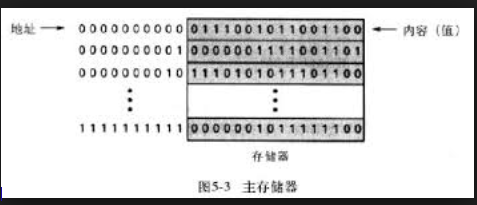
\includegraphics[width=6cm]{img/memory}
\caption{memory 逻辑图}
\label{memory}
\end{center}
\vspace{-0.5em}
\end{figure}

\end{frame}


%--------------------------------------------
\begin{frame}[fragile]{RAM and Storage }

RAM 就是内存,是一种memory ,我们常说的内存条就是这个东西。它有如下特性:
\begin{itemize}
\item 速度快。CPU 可以直接寻址。
\item 掉电数据丢失,成本高,容量小。
\end{itemize}

Storage 是 存储。 我们通常用的 磁盘,储存卡等 都归类为储存。它有如下特性:
\begin{itemize}
\item 速度慢。CPU 无法直接寻址。
\item 掉电数据不丢失,成本较低,容量大。
\end{itemize}

\end{frame}



%--------------------------------------------
\begin{frame}[fragile]{代码的执行}
写好的代码会在storage 中,被CPU 加载到 内存中,然后执行。

CPU 上电的第一条指令是再BIOS中执行。BIOS 加载 磁盘中C盘的操作系统代码到内存中。然后CPU 执行
操作系统代码。

接下来操作系统执行,加载各个系统模块,这样就有了我们电脑刚开机的样子。


\end{frame}



%========================================================================================================
\section{计算机软件架构}

%-----------------------------------------------
\begin{frame}[fragile]{要介绍的术语}

这里主要介绍 以下一些 概念
\begin{itemize}
\item bootloader 启动代码
\item 操作系统
\item 操作系统驱动
\item 操作系统应用
\item UI 和其他逻辑
\end{itemize}

\end{frame}


%-----------------------------------------------
\begin{frame}{Les listes}
	item
	\begin{itemize}
		\item Premier
		\item Second
		\item Troisième
	\end{itemize}

	枚举
	\begin{enumerate}
		\item Premier
		\item Second
		\item Troisième
	\end{enumerate}

	描述
	\begin{description}
		\item [UHA] Université de Haute Alsace
	\end{description}
\end{frame}

%-----------------------------------------------
\begin{frame}{Les blocks}
	\begin{exampleblock}{示例一}
		示例
	\end{exampleblock}
	\begin{alertblock}{提醒}
		提醒
	\end{alertblock}
	\begin{block}{普通}
		普通
	\end{block}
\end{frame}



\end{document}
